\documentclass[11pt]{amsart}

\setlength{\textwidth}{\paperwidth}
\addtolength{\textwidth}{-3in}
\calclayout

%LOAD PACKAGES--------------------------------------------

\usepackage{amsfonts, amsthm, amssymb, amsmath, stmaryrd, etoolbox}
\usepackage{comment}
\usepackage{mathtools}
\usepackage{graphicx,caption,subcaption}
\usepackage{todonotes}
\usepackage{xcolor}

\usepackage[inline]{enumitem}
\setlist{itemsep=0em, topsep=0em, parsep=0em}
\setlist[enumerate]{label=(\alph*)}

\usepackage{tikz}
\usepackage[all,2cell]{xy}
\usetikzlibrary{matrix,arrows,shapes,decorations.markings,decorations.pathreplacing}
\tikzset{->-/.style={decoration={%
			markings,
			mark=at position .5 with {\arrow{>}}},postaction={decorate}}
}
\tikzset{->-pos/.style={decoration={%
			markings,
			mark=at position #1 with {\arrow{>}}},postaction={decorate}}
}

\usepackage{hyperref}
\definecolor{hyperrefcolor}{rgb}{0,0,0.7}
\hypersetup{colorlinks,linkcolor={hyperrefcolor},citecolor={hyperrefcolor},urlcolor={hyperrefcolor}}

%NEW COMMANDS---------------------------------------------

\newcommand{\RR}{\mathbb{R}}
\newcommand{\ZZ}{\mathbb{Z}}
\newcommand{\NN}{\mathbb{N}}
\newcommand{\QQ}{\mathbb{Q}}
\newcommand{\CC}{\mathbb{C}}
\newcommand{\DD}{\mathbb{D}}
\newcommand{\MM}{\mathbb{M}}
\renewcommand{\epsilon}{\varepsilon}

\newcommand{\op}[1]{\operatorname{#1}}
\newcommand{\cat}[1]{\mathbf{#1}}
\newcommand{\dblcat}[1]{\mathbb{#1}}
\renewcommand{\t}[1]{\text{#1}}

\newcommand{\from}{\colon}
\newcommand{\xto}[1]{\xrightarrow{#1}}
\newcommand{\sm}{\smallsetminus}
\newcommand{\tospan}{\xrightarrow{\mathit{sp}}}
\newcommand{\tocospan}{\xrightarrow{\mathit{csp}}}
\newcommand{\diagram}[1]{\raisebox{-0.5\height}{\includegraphics{#1}}}

%  macros for (co)span bicategories
\newcommand{\bispmap}[1]{\mathbf{Sp(#1)}}
\newcommand{\dblspmap}[1]{\mathbb{S}\mathbf{p(#1)}}
\newcommand{\bicspmap}[1]{\mathbf{Csp(#1)}}
\newcommand{\dblcspmap}[1]{\mathbb{C}\mathbf{sp(#1)}}
\newcommand{\bispsp}[1]{\mathbf{Sp(Sp(#1))}}
\newcommand{\dblspsp}[1]{\mathbb{S}\mathbf{p(Sp(#1))}}
\newcommand{\bicspcsp}[1]{\mathbf{Csp(Csp(#1))}}
\newcommand{\dblcspcsp}[1]{\mathbb{C}\mathbf{sp(Csp(#1))}}
\newcommand{\bimonspcsp}[1]{\mathbf{MonicSp(Csp(#1))}}
\newcommand{\dblmonspcsp}[1]{\mathbb{M}\mathbf{onicSp(Csp(#1))}}
\newcommand{\biepiccspsp}[1]{\mathbf{EpicCsp(Sp(#1))}}
\newcommand{\dblepiccspsp}[1]{\mathbb{E}\mathbf{picCsp(Sp(#1))}}

% defining arrow with a vertical line through it
\makeatletter
\def\slashedarrowfill@#1#2#3#4#5{%
	$\m@th\thickmuskip0mu\medmuskip\thickmuskip\thinmuskip\thickmuskip
	\relax#5#1\mkern-7mu%
	\cleaders\hbox{$#5\mkern-2mu#2\mkern-2mu$}\hfill
	\mathclap{#3}\mathclap{#2}%
	\cleaders\hbox{$#5\mkern-2mu#2\mkern-2mu$}\hfill
	\mkern-7mu#4$%
}
\def\rightslashedarrowfill@{%
	\slashedarrowfill@\relbar\relbar\mapstochar\rightarrow}
\newcommand{\xslashedrightarrow}[2][]{%
	\ext@arrow 0055{\rightslashedarrowfill@}{#1}{#2}}
\makeatother

\newcommand{\hto}{\xslashedrightarrow{}}


%DECLARE MATH OPERATORS----------------------------------

\DeclareMathOperator{\Hom}{Hom}
\DeclareMathOperator{\id}{id}
\DeclareMathOperator{\ob}{Ob}
\DeclareMathOperator{\arr}{arr}
\DeclareMathOperator{\im}{im}
\DeclareMathOperator{\Aut}{Aut}
\DeclareMathOperator{\Bij}{Bij}
\DeclareMathOperator{\Sub}{Sub}

%ENVIRONMENTS AND COUNTERS---------------------------------

\newtheorem{thm}{Theorem}[section]
\newtheorem{lem}[thm]{Lemma}
\newtheorem{prop}[thm]{Proposition}
\newtheorem{cor}[thm]{Corollary}

\theoremstyle{remark}
\newtheorem{remark}[thm]{Remark}
\newtheorem{notation}[thm]{Notation}

\theoremstyle{definition}
\newtheorem{ex}[thm]{Example} 
\newtheorem{defn}[thm]{Definition}

%\setcounter{tocdepth}{1} % Sets depth for table of contents. 

%%%%%%%%%%%%%%%%%%%%%%%%%%%%%%%%%%%%%%%%%%%%%%%%%%%%%%%%%
%%%%%%%%%%%%%%%%%%%%%%%%%%%%%%%%%%%%%%%%%%%%%%%%%%%%%%%%%
%%%%%%%%%%%%%%%%%%%%%%%%%%%%%%%%%%%%%%%%%%%%%%%%%%%%%%%%%
%%%%%%%%%%%%%%%%%%%%%%%%%%%%%%%%%%%%%%%%%%%%%%%%%%%%%%%%%
%
%BEGIN DOCUMENT
%
%%%%%%%%%%%%%%%%%%%%%%%%%%%%%%%%%%%%%%%%%%%%%%%%%%%%%%%%%
%%%%%%%%%%%%%%%%%%%%%%%%%%%%%%%%%%%%%%%%%%%%%%%%%%%%%%%%%
%%%%%%%%%%%%%%%%%%%%%%%%%%%%%%%%%%%%%%%%%%%%%%%%%%%%%%%%%
%%%%%%%%%%%%%%%%%%%%%%%%%%%%%%%%%%%%%%%%%%%%%%%%%%%%%%%%%

\begin{document}
	
Let's recast the 
reachability problem 
of Petri nets
as a question about 
2-cells.
First, we realize
a marked Petri net $P$
as a 1-cell in 
$\cat{MonSp(Csp(C))}$
for a suitable category $\cat{C}$.
Note, this realization
is inspired by the fact 
that a marked Petri net 
can be thought of as a multiset.

Let $P_S$ be the set of species
for $P$.  A marking of $P$ is a
map $m \from X \to P_S$ for some
finite set of tokens $X$. 

Since $\cat{FinSet}$ is a topos
and topoi are closed under
taking slice categories,
we can consider the bicategory
$\cat{MonSp ( Csp ( FinSet / P_S ) ) }$.
Call this $\cat{B}$ for short.
To refresh your memory,
this is the bicategory 
[finite sets over $P_S$,
cospans of finite sets over $P_S$,
monic spans of cospans of finite sets over $P_S$]

We are interested in the hom-category 
$\cat{B}( \emptyset , \emptyset )$,
where $\emptyset$ is taken over $P_S$
in the only way possible.
This category is just
[ finite sets over $P_S$,
 monic spans of finite sets over $P_S$ ]
But a finite set over $P_S$, 
say $f \from X \to P_S$, 
is really a multiset where
$s \in P_S$ has multiplicity
$| f^{-1} ( s ) |$.
We want spans of finite sets over $P_S$ 
to correspond to a transformation
from one marking of $P_S$ to another.
So the entire structure of 
$\cat{B}( \emptyset , \emptyset )$
is giving us the collection of 
all markings of $P_S$ for objects
and allowing any marking to
be transformed into any other marking,
which is clearly not what we want.
So we should consider a subcategory
corresponding to the trasitions
of the Petri net $P$.

Here's an illustration.  
Consider the Petri net $P$
 \[
 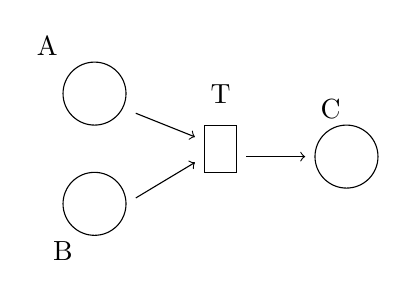
\begin{tikzpicture}
 \draw  (-0.6,0.6) ellipse (0.4 and 0.4);
 \draw  (-0.6,-0.8) ellipse (0.4 and 0.4);
 \draw  (2.6,-0.2) ellipse (0.4 and 0.4);
 \draw  (0.8,0.2) rectangle (1.2,-0.4);
 \node (v1) at (-0.2,0.4) {};
 \node (v2) at (0.8,0) {};
 \node (v3) at (-0.2,-0.8) {};
 \node (v4) at (0.8,-0.2) {};
 \node (v5) at (1.2,-0.2) {};
 \node (v6) at (2.2,-0.2) {};
 \draw [->] (v1) edge (v2);
 \draw [->] (v3) edge (v4);
 \draw [->] (v5) edge (v6);
 \node at (-1.2,1.2) {A};
 \node at (-1,-1.4) {B};
 \node at (2.4,0.4) {C};
 \node at (1,0.6) {T};
 \end{tikzpicture}
 \]
We have species $A,B,C$ and 
transitition $T$. 
All the possible markings
of $P$ are given by maps
$f \from X \to \{A,B,C\}$ where 
$X$ is some finite set
of tokens and the number
of tokens in, say, $A$ is $ |f^{-1} (A)|$.
The transition we have takes
an $A$ token and a $B$ token 
and turns it to a $C$ token.  
We can think of this like a span
\[
	\{A,B\} \gets \emptyset \to \{C\}.
\]
This translates into the 
bicategory by looking at the 
hom-category
$ \cat{B} ( \emptyset , \emptyset ) $
with all objects, the cospans
\[
	\emptyset \gets X \to \emptyset
\]
for finite sets $X$ over $P_S$ 
(corresponding to all possible markings)
and a single generating morphism
(corresponding to the single 
transition $T$)
\[
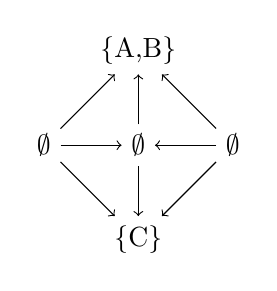
\begin{tikzpicture}
\node (v1) at (-1,-2.2) {$\emptyset$};
\node (v2) at (0.2,-1) {\{A,B\}};
\node (v3) at (0.2,-2.2) {$\emptyset$};
\node (v4) at (0.2,-3.4) {\{C\}};
\node (v5) at (1.4,-2.2) {$\emptyset$};
\draw [->]  (v1) edge (v2);
\draw [->] (v1) edge (v3);
\draw [->] (v1) edge (v4);
\draw [->] (v5) edge (v2);
\draw [->] (v5) edge (v3);
\draw [->] (v5) edge (v4);
\draw [->] (v3) edge (v2);
\draw [->] (v3) edge (v4);
\end{tikzpicture}
\]

So the reachability problem
is reduced to asking whether
a certain span of cospan exists.

Natural questions are what other
hom-categories correspond to 
in this context. 
I think it fixes a number of tokens
that cannot be transfered
under any rewriting.  
So it seems like something
of a context in which
a rewrite can happen.  
But a bit more subtle
than this too, so 
it's worth some thought.










%%%%%%%%%%%%%%%%%%%%%%%%%%%%%%%%%%%%%%%%%%%%%%%%%%%%%%%%%
%%%%%%%%%%%%%%%%%%%%%%%%%%%%%%%%%%%%%%%%%%%%%%%%%%%%%%%%%
%%%%%%%%%%%%%%%%%%%%%%%%%%%%%%%%%%%%%%%%%%%%%%%%%%%%%%%%%
%%%%%%%%%%%%%%%%%%%%%%%%%%%%%%%%%%%%%%%%%%%%%%%%%%%%%%%%%
%
%END DOCUMENT
%
%%%%%%%%%%%%%%%%%%%%%%%%%%%%%%%%%%%%%%%%%%%%%%%%%%%%%%%%%
%%%%%%%%%%%%%%%%%%%%%%%%%%%%%%%%%%%%%%%%%%%%%%%%%%%%%%%%%
%%%%%%%%%%%%%%%%%%%%%%%%%%%%%%%%%%%%%%%%%%%%%%%%%%%%%%%%%
%%%%%%%%%%%%%%%%%%%%%%%%%%%%%%%%%%%%%%%%%%%%%%%%%%%%%%%%%

\end{document}
